
%
%  $Description: Author guidelines and sample document in LaTeX 2.09$ 
%
%  $Author: ienne $
%  $Date: 1995/09/15 15:20:59 $
%  $Revision: 1.4 $
%

\documentclass[times, 10pt,twocolumn]{article} 
\usepackage{latex8}
\usepackage{times}
\usepackage{graphicx}
\usepackage{enumerate}
\usepackage{amsmath}
\usepackage{url}



%\documentstyle[times,art10,twocolumn,latex8]{article}

%------------------------------------------------------------------------- 
% take the % away on next line to produce the final camera-ready version 
\pagestyle{empty}

%------------------------------------------------------------------------- 
\begin{document}

\title{VMKit - Adaptive Optimization System  for LLVM JIT Compiler}

\author{
Gayana Ranganatha Chandrasekara Pilana Withanage,Kuganesan Srijeyanthan, David Daharewa Gureya\\
\{gayana.withanage, kuganesan.srijeyanthan, david.gureya \} @tecnico.ulisboa.pt\\
Group 2- Virtual Execution Environments: 79529, 79531, 79533\\
\textbf{\textit{Instituto Superior T\'{e}cnico, Lisbon, Portugal.}}\\
March 2014\\
% For a paper whose authors are all at the same institution, 
% omit the following lines up until the closing ``}''.
% Additional authors and addresses can be added with ``\and'', 
% just like the second author.
}

\maketitle
\thispagestyle{empty}

\begin{abstract}
This article is presented to propose an improvement for an existing problem regarding the performance of LLVM JIT (Just in Time) compiler, which is an inherent slowness during the start-up of virtual machines (VM), Ex: VMKit ~\cite{arch1}. Our proposed solution is to use a Trace based JIT compiler as an adaptive optimization for the current LLVM JIT.  Moreover our implementation will have a mixed mode execution including a byte-code interpreter and LLVM JIT together. In the end, we will benchmark our implementation so that we can compare the difference in performance of the current LLVM JIT and the improved LLVM JIT with VMKit framework.\\
 \textbf{\textit{Key words}}:  VMKit, LLVM, JIT, VM
\end{abstract}


%------------------------------------------------------------------------- 
\Section{Overview}
\label{sec:introduction}

Implementing a virtual machine (VM) is a painful task which demands huge effort and knowledge regarding the hosting infrastructure and architecture. When moving from one architecture to the other it is again a time consuming task which demands reimplementation of the main modules of VM. To relax this inherent overhead of building a VM, VMKit which work as a substrate has been developed so that it provides about 95 percent of the code required in developing a new VM. VMKit provides basic components required to create a VM such as JIT (Just In Time) compiler, Garbage Collector (GC) and a Thread Manager.\\
J3 and N3 are VMs that have been developed using VMKit which prove the significant reduction in development time of a completely new VM ~\cite{arch1}. Furthermore, the core of VMKit depends on LLVM compiler infrastructure which provides the required key components such as JIT compiler and GC. In this article our point of interest is the LLVM JIT compiler because it is a known fact that the startup time consumption during the VM execution, developed using this core module is considerably higher. Therefore we propose an improvement for the behavior of LLVM JIT compiler, in order to make the startup and the run time to be faster than the current implementation. 


%------------------------------------------------------------------------- 
\Section{Virtualization technology studied }
\label{sec:related}
\begin{itemize}
 \item  \textbf{\textit{Name}}: VMKit
 \item  \textbf{\textit{URL}}: http://vmkit.llvm.org/
 \item  \textbf{\textit{VM-type}}: High Level Language VM
 \item  \textbf{\textit{Common usage}}: VMKit eases the development of new managed runtime environments (MREs) and the process of experimenting with new mechanisms inside MREs. J3(JVM) and N3(CLI) are built on top of VMKit.
\item  \textbf{\textit{Motivation}}: While VMKit aims to provide a fully functional intermediate layer for VM, it’s still under heavy development and misses some vital components with some open projects proposed. One of the current drawbacks of the LLVM JIT is the lack of an adaptive compilation system which will be our contribution to this project. What is missing is a system that can keep track of and dynamically look-up the hotness of methods and re-compile with more expensive optimizations as the methods are executed over and over. This should improve program startup time and execution time and will bring great benefits to overall performance.
\end{itemize}



%------------------------------------------------------------------------- 
% \Section{Internal Mechanisms Study -JIT compilation with LLVM}


\Section{VMKit}
\label{sec:concurrency}
VMKit is a common substrate that eases the development of new managed runtime environments (MREs) and the process of experimenting with new mechanisms inside MREs.
It provides the following to the end users: a precise garbage collection, Just-In-Time and Ahead-of-Time compilation and portability on many architectures. For the MRE developer, VMKit provides: research and development infrastructure for virtual machines and a relatively small code base. The main goal of the VMKit is to help experiments on virtual machines.

VMKit uses  LLVM as the JIT compiler (generates the native code on the fly), MMTk as the memory manager (allocating and collecting free memory automatically) and POSIX Threads as the thread manager (creating and synchronizing threads).

\begin{figure}[ht!]
\centering
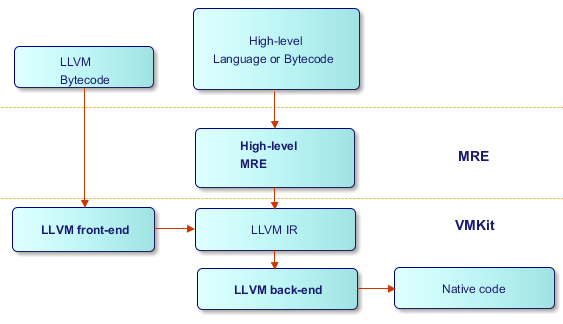
\includegraphics[width=80mm]{vmkitcompilation.png}
\caption{Compilation process in VMKit}
\label{fig:vmkitimplementation}
\end{figure}

\subsection{The JIT Compiler}

The LLVM Project is a collection of modular and reusable compiler and tool chain technologies. All the libraries including VMKit have been implemented in C++. As VMKit is a substrate for VMs, the components integrated in order to develop VMKit should have a general purpose interfaces and functionalities. Therefore the compiler should have support for a general purpose instruction set to allow VMs to implement intermediate representations of arbitrary functions. LLVM JIT is exactly a suitable compiler for this task because of its inherent behavior without  imposing object model or type system.\\
Once the VM generates the intermediate representation (IR) with the help of interfaces provided by LLVM, that VM delegates the compilation to LLVM JIT to generate the native code. LLVM JIT optimizes all methods to the same degree without considering the frequency of the number of time each method get called. This behavior is called the compilation without adaptive optimization. As a result, the initialization time get higher and the runtime also shows some slowness.\\
The LLVM IR is made up five instructions (i) arithmetic, copy and cast operations on registers, (ii) local control flow instructions (branch), (iii) method invocation (direct and indirect), (iv) memory reads and writes and (v) intrinsics.\\

\begin{figure}[ht!]
\centering
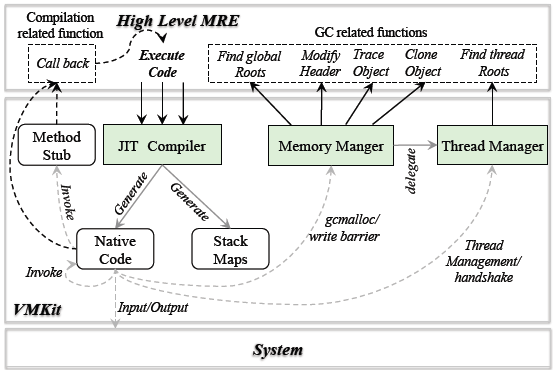
\includegraphics[width=80mm]{vmkit.png}
\caption{VMKit architecture}
\label{fig:vmkitimplementation}
\end{figure}

\subsection{Compiler extension with  intrinsics}
Any language should be able to map to the LLVM IR. Since LLVM directly targets the C language, there are many instructions that are not extensible in C that could be used by MREs, e.g. atomic instructions. LLVM supports this instructions by means of intrinsics: an intrinsic is a contract between the language and the compiler to generate a specific assembly instruction. It is materialized as a function call in LLVM. Beside atomic instructions there are other processor instructions, like vector operations, math operations and stack operations that LLVM implement as intrinsics.

\subsection{Lazy Compilation}
The execution engine performs lazy compilation of the methods throughout the lifetime of the application i.e. in case a method calls another method which has not been translated or compiled yet, the execution engine inserts a callback. When called, the callback invokes the high-level MRE method to locate the new method.The high-level MRE provides the callback function. It loads and generates the intermediate representation of the lazily compiled function, and finally delegates to LLVM the generation of its native representation. Once the function is generated, LLVM patches the calling site to call the newly generated function for subsequent calls.

%  presented trace-based JIT compilation as an adaptive optimization method for LLVM which is the technique used by virtual machines to optimize the execution of a program at runtime. Our implementation uses a hybrid mode of execution approach: the VMKit starts running in a fast-starting byte-code interpreter. As the program runs, the VMKit identifies hot (frequently executed) byte-code sequences, records them, and compiles them to fast native code. This method will be called as sequence of instruction, a trace. We have made this design decision which is based on the assumptions that program are spend most of their time in hot loops. Further, trace-based JIT can greatly speed up programs if they spend most of their time in loops where they take similar code paths.
%------------------------------------------------------------------------- 
\Section{Detail Sections}
\label{sec:architecture}
Loops are not compiled the first time they are called. VMKit maintains a loop count,which is incremented every time the loop executed.  VM interprets a loop until its call count exceeds a predefined trace\_JIT threshold value. So, most frequent loops(hot) are compiled as soon as VM started, loops which are executing less than threshold value will not be compiled by JIT. The threshold value could be selected to obtain significant balance between start-up times and run-time performance.\\
After particular loop is compiled, its call count will be reset to zero. Subsequent calls to the loop continue to increment its count. When the call count reaches its trace\_JIT threshold again it will be compiled by applying more optimization methods. This scenario will be occurred on some methods during an aggressive call by VM. So, high frequent loops will be more optimized than the normal less frequent routine.

\begin{figure}[ht!]
\centering
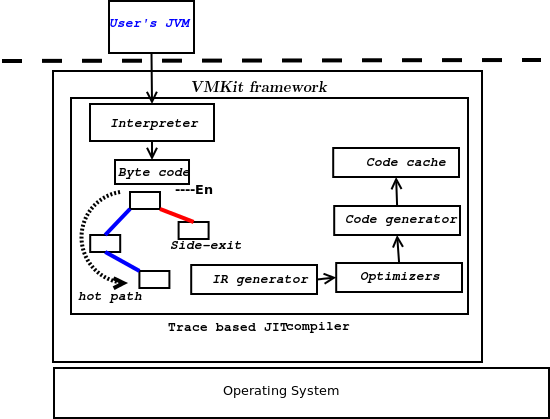
\includegraphics[width=70mm]{compiler.png}
\caption{Trace based JIT for VMKit}
\label{fig:architecture}
\end{figure}

Fig 1 explains how trace based JIT will lay down in VMKit. Even though VMKit composed with other components , diagram shows only JIT components which has derived from LLVM. As number of loop execution is counting by JIT when the counter reaches a threshold, the interpreter will be starting trace process. According to above diagram tracing process will be started at place -En and when tracing process reaches  back to the address where the tracing started, the interpreter stops tracing and the compiler compiles the trace to native code. The path in blue may or may not be an actual hot path since interpreter is not doing an perfect path profiling. Guard control will be applied when instructions are deviated from actual hot path. During the interpretation , if a Guard is triggered , the native code use side-exit and back to normal interpretation mechanism. There are some other advanced way to deal with frequent side-exit which would make side-exit path to separate branch of hot-path ~\cite{arch2}.


%------------------------------------------------------------------------- 
\Section{Conclusion}
\label{sec:conclusion}

VMKit provides a substrate for the development of VMs within a short period of time but still it has left interesting research areas in optimizing the execution of the VMs. Therefore our proposed solution for the LLVM JIT improvement would be an exciting research area to identify and exercise Virtualization concepts in practice.
At the checkpoint level, we hope to have a thorough understanding of the current system architecture and a prototype version of our implementation which will provide a better insight of the system behaviour. Finally, at the successful completion of this project we are hoping to contribute our research efforts to the VMKit community


%------------------------------------------------------------------------- 

\bibliographystyle{plain}
\bibliography{latex8.bib}

\end{document}

